\documentclass{article} % Tipo de documento

\usepackage[utf8]{inputenc} % Permite el uso de caracteres del Español

\usepackage[T1]{fontenc}

\usepackage{graphicx}

% Carátula del Artículo  

\title{Reporte de Actividad 2}

\author{Brenda Leyva Amaya}

\date{07 de febrero, 2018}
 

\begin{document}

\maketitle % Crea el título


\section{Introducción}

	Esta actividad tiene como fin el introducirnos al lenguaje de programación Python y las distintas herramientas que se pueden utilizar para manejo de datos numéricos y graficación de los mismos. Este primer contacto nos ayudará a ir identificando los usos que podremos darle a la programación en este lenguaje y las posibilidades que se abren, así mismo poder entender las similitudes entre Fortran y Python que hasta ahora son los lenguajes con los cuales hemos estado trabajando. 
\vspace{0.5 cm}
En general es importante esta nueva actividad pues Python es un lenguaje que se utiliza más ampliamente en las diferentes actividades que se realizan en programación no sólo con fines científicos si no también como herramienta en las diferentes empresas donde se desarrolla nueva tecnología, por ello que sea de gran utilidad para nosotros como estudiantes adquirir este tipo de habilidades. 

\section{Jupyter Notebook.}
Jupyter Notebook es un entorno de programación que permite una combinación inmediata de la creación de código, la compilación y el uso de herramientas matemáticas y gráficas para la manipulación de información. 
\vspace{0.5 cm}
La ventaja principal de esta herramienta es la experiencia de usuario, es un ambiente altamente amigable con el usuario y permite interactuar con el lenguaje de programación Python de una manera sencilla y ordenada. 
\vspace{0.5 cm}
En este primer acercamiento al área de trabajo de Jupyter Notebook no se han identificado aún ningún tipo de desventajas. De hecho, la experiencia ha sido muy positiva y es una manera muy sencilla de comenzar a utilizar un lenguaje de programación pues inmediatamente después de configurar un segmento de código se puede ver el resultado que se tendrá al compilar. 


\section{Biblioteca Pandas de Python.}
Pandas es un paquete que se puede utilizar con el lenguaje Python, este provee de estructuras de datos rápidas, flexibles y expresivas, diseñadas para hacer fácil e intuitivo el trabajo con datos en relaciones y etiquetado. Su meta es ser el bloque constructor fundamental y alta calidad para realizar análisis de datos basado en la vida real con Python. Adicionalmente en el futuro la meta es convertir pandas en la principal herramienta de manipulación de datos para cualquier otro lenguaje.
\vspace{0.5 cm}
En la presente actividad utilizamos la biblioteca pandas y una serie de datos meteorológicos, esto nos permitió realizar una serie de análisis gráficos para describir la fenomenología que se presentaba, basado en las distintas mediciones que se tenían en la base de datos correspondiente. 


\section{Productos de la Actividad 2.}
Primeramente se obtuvo un visual de de la manera en que varía la rapidez de los vientos, el lugar observado es Rosarito, Baja California. Como se puede ver aquí abajo la gráfica obtenida es de buena calidad y se obtuvo gracias al uso de la biblioteca Pandas con un segmento muy sencillo de código.
 \begin{center}
 	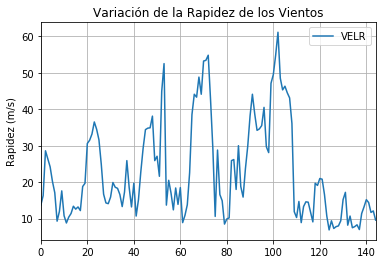
\includegraphics[width=8cm]{1.png}
 \end{center}

A continuación obtuvimos un gráfico correspondiente a la manera en que varían la Temperatura y la Humedad Relativa. Aquí por primera vez utilizamos la grafiación de dos series de datos, y pudimos observar la facilidad con la cual podemos modificar estéticamente el gráfico respecto a sus colores y etiquetas.

 \begin{center}
 	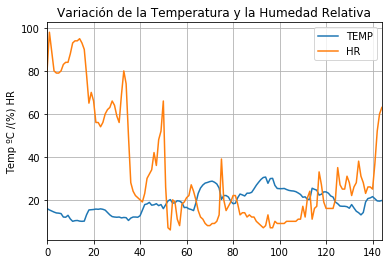
\includegraphics[width=8cm]{2.png}
 \end{center}

La imagen abajo muestra la variación de la temperatura en el lugar seleccionado, todas y cada una de las gráficas generadas en esta actividad responden  a un pequeño segmento de código de estructura simple y fácil de replicar.

 \begin{center}
 	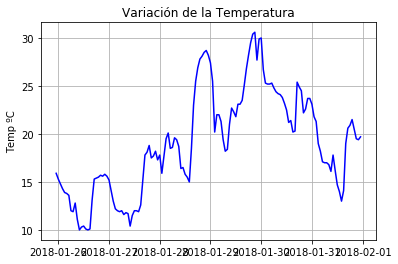
\includegraphics[width=8cm]{3.png}
 \end{center}

De la misma manera que se mencionó en el caso anterior donde trabajábamos datos de dos series distintas, utilizando otros colores y diferentes etiquetas. 

 \begin{center}
 	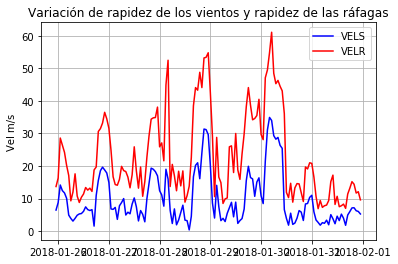
\includegraphics[width=8cm]{4.png}
 \end{center}

A continuación se hizo un análisis de la dirección de los vientos con respecto al tiempo.

 \begin{center}
 	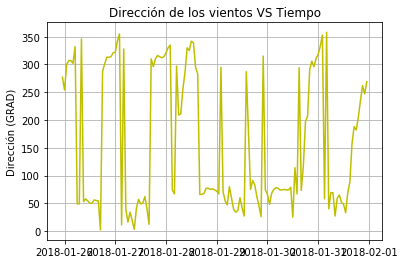
\includegraphics[width=8cm]{5.png}
 \end{center}

Finalmente generamos con los datos proporcionados en la base de datos, un visual de los niveles de radiación solar y su variación respecto al tiempo.

 \begin{center}
 	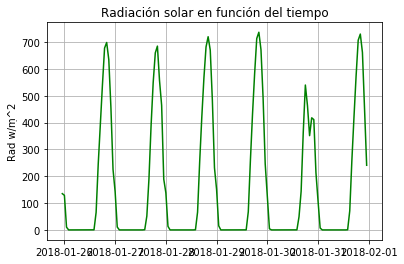
\includegraphics[width=8cm]{6.png}
 \end{center}


\section*{Apéndice:}
\hspace{0.45 cm} ¿Cuál es tu primera impresión de Jupyter Notebook?

\vspace{0.5 cm}

** El entorno de Jupyter es altamente funcional y agradable, es ideal para comenzar a utilizar un nuevo lenguaje de programación pues la interacción del código y la compilación es en tiempo real.

\vspace{0.5 cm}

¿Se te dificultó leer código en Python?

\vspace{0.5 cm}

** No, los comandos o instrucciones utilizados son bastante claros y llevan un orden muy lógico como debe ser una buena programación en cualquier lenguaje. 

\vspace{0.5 cm}

¿En base a tu experiencia de programación en Fortran, que te parece el entorno de trabajar en Python?

\vspace{0.5 cm}

** La primera impresión de python es muy positiva y lleva a pensar que es un lenguaje mucho más amistoso con el programador que Fortran, esta opinión parece estar muy influenciada en que el lenguaje se utiliza por primera vez en Jupyter que es bueno para quien no es experto en programación.

\vspace{0.5 cm}

A diferencia de Fortran, ahora se producen las gráficas utilizando la biblioteca Matplotlib. ¿Cómo fue tu experiencia?. 

\vspace{0.5 cm}

** En general es mucho más sencillo interactuar con el nuevo lenguaje y con las herramientas que se utilizaron para la manipulación de la información.

\vspace{0.5 cm}

En general, ¿qué te pereció el entorno de trabajo en Python? 

\vspace{0.5 cm}

** Excelente, me gustaría continuar aprendiendo y mejorando el uso del lenguaje y el entorno de programación que utilizamos en esta actividad pues parecen mucho más rápidos y eficientes que la generación de código en Fortran.

\vspace{0.5 cm}

¿Qué opinas de la actividad? ¿Estuvo compleja? ¿Mucho material nuevo? ¿Que le faltó o que le sobró? ¿Qué modificarías para mejorar? 

\vspace{0.5 cm}

** La actividad me pareció ideal para una primera aproximación a Python, no le agregaría ni quitaría nada en realidad pues me agradó mucho, quizá un par de acciones más que ayuden a explorar la capacidad de las bibliotecas para realizar cálculos.

\vspace{0.5 cm}

¿Comentarios adicionales que desees compartir?

\vspace{0.5 cm}

** Una vez terminada esta actividad me encuentro suficientemente motivada a seguir trabajando con las herramientas que se nos presentaron y además de ir conociendo nuevas para poder aplicarlas a diferentes aspectos tanto escolares como personales. 

\vspace{0.5 cm}

 
\end{document}